\documentclass[a4paper,12pt]{ctexart}
\usepackage[utf8]{inputenc}
\usepackage{geometry}
\usepackage{amsmath}
\usepackage{amssymb}
\usepackage{graphicx}
\usepackage{fancyhdr}
\usepackage{tcolorbox}

% 页面设置
\geometry{left=2.5cm,right=2.5cm,top=2.5cm,bottom=2.5cm}
\pagestyle{fancy}
\fancyhf{}
\lhead{高频电子线路}
\rhead{期末真题/模拟题精选}
\cfoot{\thepage}

\title{\textbf{高频电子线路：期末复习精选试题}\\ \large{完全契合复习考纲}}
\author{23届陈文斗}
\date{\today}

\begin{document}

	\maketitle

	\begin{tcolorbox}[colback=blue!5!white,colframe=blue!75!black,title=说明]
		本试题集根据上传的试卷图片整理，覆盖了调制概念、振荡器判别、阻抗匹配、功率放大器及小信号放大器等核心考点。建议作为考前模拟自测使用。
	\end{tcolorbox}

	\section*{一、 系统概念与基本原理（18分）}
	\textbf{题目描述：}
	下图（需参考原卷框图）为无线电对讲机系统框图，请分析描述框图中每一个模块的功能。这些模块包括：调制器、载波振荡器、变频器、激励放大器、功率放大器 PA、天线开关、高频小信号放大器 LNA、混频器 Mixer、本地振荡器、中频放大器与滤波和解调器。

	\textbf{简答题：}
	\begin{enumerate}
		\item 什么是调制（定义）？
		\item 无线电通信系统为什么要调制？
		\item 目前音频模拟调制系统有哪些调制方式？请举例列出至少两种。
		\item 接收机为什么需要混频？混频的好处是什么？
	\begin{center}
		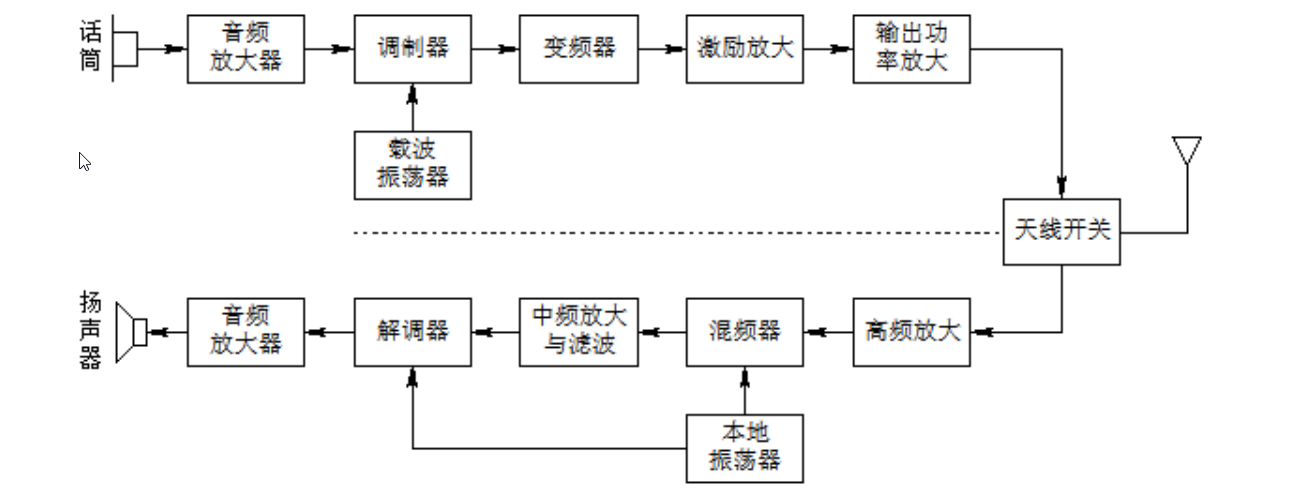
\includegraphics[width=0.8\textwidth]{14-30.png}
	\end{center}
	\end{enumerate}

	\newpage

	\section*{二、 振荡器判别（12分）}
	\textbf{题目描述：}
	下图是三端式正弦波振荡器的等效电路，设有下列四种情况：
	\begin{itemize}
		\item[(1)] $L_1 C_1 = L_2 C_2 > L_3 C_3$
		\item[(2)] $L_1 C_1 > L_2 C_2 > L_3 C_3$
		\item[(3)] $L_1 C_1 < L_2 C_2 = L_3 C_3$
		\item[(4)] $L_1 C_1 < L_2 C_2 < L_3 C_3$
	\end{itemize}
	\begin{center}
		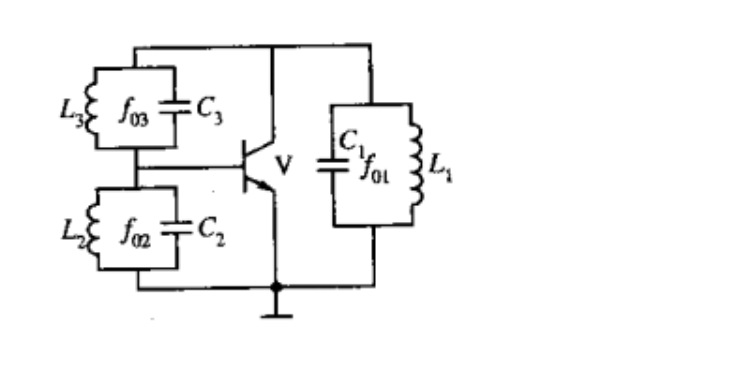
\includegraphics[width=0.8\textwidth]{14-33.png}
	\end{center}
	试分析上述四种情况是否都能振荡。若能振荡，振荡频率 $f$ 与回路谐振频率有何关系？其中 $f_{01}, f_{02}, f_{03}$ 分别是三谐振回路的谐振频率。并说明是何种类型的三端式振荡器？

	\newpage
	\section*{三、 LC 串联谐振回路计算（10分）}
	\textbf{题目描述：}
	已知 LC 串联谐振回路 $f_0 = 10 \text{ MHz}$，$C_0 = 120 \text{ pF}$，谐振时电阻为 $R = 4 \Omega$。
	\begin{enumerate}
		\item 试求 $Q_0$ 和 $L_0$。
		\item 又若已知信号源电压振幅 $V_{SM} = 120 \text{ mV}$，求谐振时回路中的电流振幅 $I_0$ 以及电感、电容上的电压峰值 $V_{LM}$ 和 $V_{CM}$。
	\end{enumerate}

	\newpage
	\section*{四、 阻抗匹配网络设计（10分）}
	\textbf{题目描述：}
	已知传输线的特性阻抗为 $Z_0 = 50 \Omega$，射频芯片的工作频率为 $315 \text{ MHz}$，RF 芯片的射频信号输出端的输出阻抗 $R_e = 500 \Omega$。
	请设计一 L 型阻抗匹配网络（电路）将传输线与射频芯片口相连，实现信号最大功率传输。
	\begin{center}
		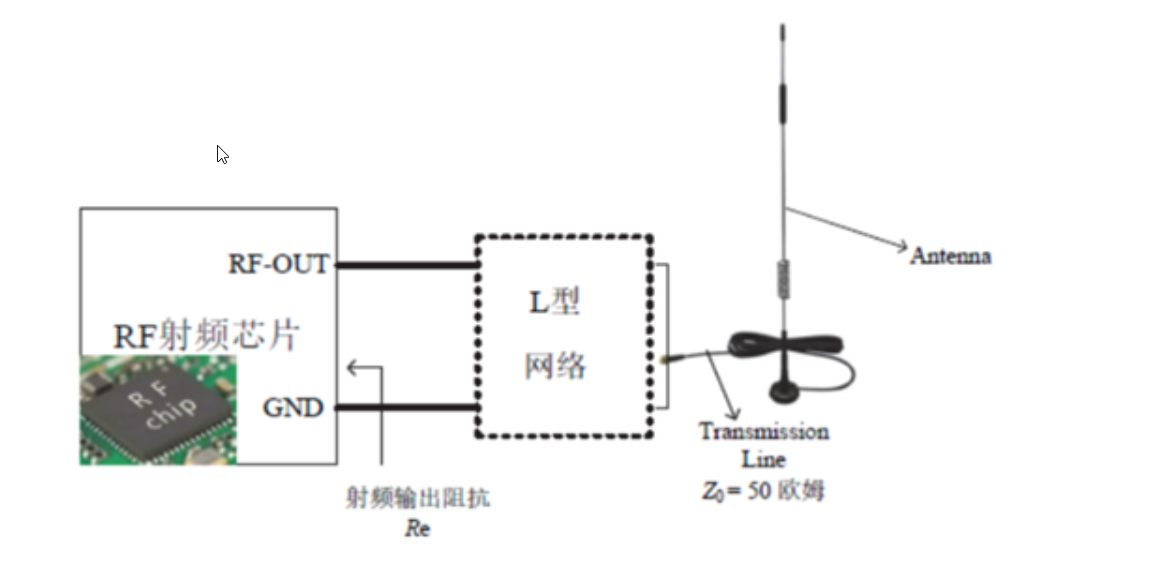
\includegraphics[width=0.8\textwidth]{14-36.png}
	\end{center}
	\begin{itemize}
		\item 提示：画出电路结构并计算 $L$ 和 $C$ 的值。
	\end{itemize}

	\newpage
	\section*{五、 统调与垫整电容计算（10分）}
	\textbf{题目描述：}
	下图为收音机用于波段内调台使用的并联谐振回路，可变电容 $C$ 的变化范围为 $30 \sim 555 \text{ pF}$，$C_t$ 为微调电容。要求此回路的调谐范围为 $4.25 \sim 17 \text{ MHz}$。
	求回路电感 $L$ 和 $C_t$ 的值（要求 $C$ 的最大和最小值与波段的最低和最高频率对应）。
	\begin{center}
		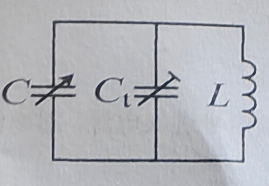
\includegraphics[width=0.8\textwidth]{14-38.png}
	\end{center}
	\newpage
	\section*{六、 高频功率放大器综合分析（20分）}
	\textbf{题目描述：}
	下图是一个实际的高频功率放大电路，包括激励级与输出级。
	\begin{enumerate}
		\item 根据框图阐述各模块由哪些元件构成？各模块的功能作用是什么？
		\item 激励级和输出级的工作状态如何？供电与偏置电路由哪些元件构成？
		\item 若此功放输出功率为 $40 \text{ dBm}$，则输出功率为多少 W？若功率放大增益为 $20 \text{ dB}$，则功率放大增益比值为多少？
		\item 已知晶体管 $Q_2$ 的输出阻抗为 $(5 - j10) \Omega$，隔直电容 $C_4$ 为 $1061 \text{ pF}$，工作频率为 $30 \text{ MHz}$，试计算阻抗匹配网络 $L_5$ 和 $C_5$ 的值
	\begin{center}
		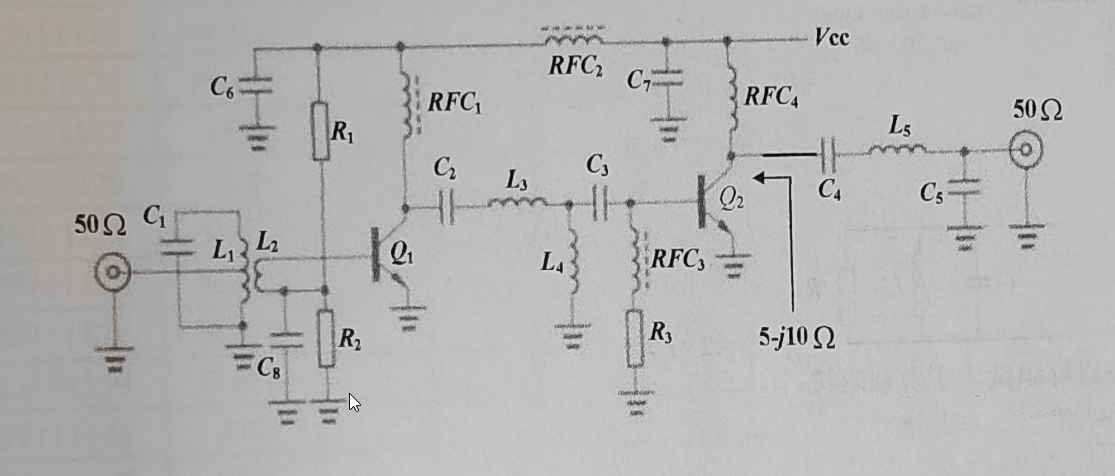
\includegraphics[width=0.8\textwidth]{power_amplifier1.png}
	\end{center}
	\end{enumerate}

	\newpage
	\section*{七、 高频小信号放大器（20分）}
	\textbf{题目描述：}
	某调谐放大器如下图所示，$f_0 = 6.5 \text{ MHz}$。中频变压器 $L_{13} = 5.8 \text{ uH}$，$Q_0 = 80$，匝数比 $n_{13} = 20T, n_{23} = 8T, n_{45} = 5T$，初次级为紧耦合。
	两级晶体管的工作点相同，在工作点和工作频率上测得它们的参数为：
	$g_{ie} = 2860 \text{ uS}, C_{ie} = 32 \text{ pF}, g_{oe} = 200 \text{ uS}, C_{oe} = 2 \text{ pF}, |y_{fe}| = 45 \text{ mS}, y_{re}$ 可忽略。
	试画出其高频小信号等效电路，并计算谐振电容 $C$ 的值、通频带 $BW$ 和放大器的功率增益 $G_p = P_{i2}/P_{i1}$。（上述计算中可忽略偏置电阻的影响）。
	\begin{center}
		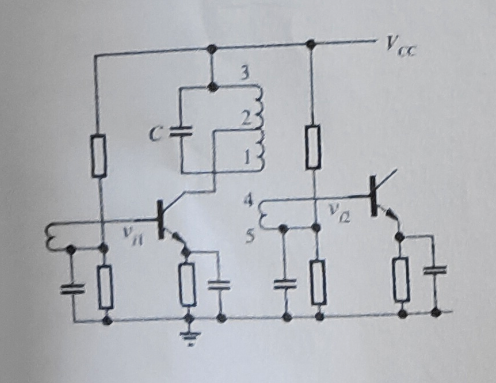
\includegraphics[width=0.8\textwidth]{14-40.png}
	\end{center}
	\newpage

	\section*{八、 查漏补缺：考纲特别补充题（$\bigstar$ 考前必看）}

	\textbf{补充题 1：AD630 与开关函数调制（对应手写考纲“AD630”）}
	\begin{itemize}
		\item \textbf{题目描述}：AD630 是一款基于\textbf{开关函数法}（Switching）的平衡调制/解调器。
		\item \textbf{问题}：
		\begin{enumerate}
			\item AD630 内部通过比较器将载波信号转化为方波（开关函数 $K(t)$），其取值为 $+1$ 或 $-1$。若输入信号为 $v_i(t) = V_{im}\cos(\Omega t)$，请写出输出信号 $v_o(t)$ 的时域表达式（用 $v_i(t)$ 和开关函数级数展开式表示）。
			\item \textbf{简答}：相比于模拟乘法器（如 MC1496），利用开关函数进行调制/解调的主要优点是什么？（提示：通常与动态范围、温漂或线性度有关）。
		\end{enumerate}
	\end{itemize}

	\newpage
	\textbf{补充题 2：丙类功放的负载特性分析（对应考纲“状态分析”）}
	\begin{itemize}
		\item \textbf{题目描述}：某丙类谐振功率放大器原工作在\textbf{临界状态}。保持电源电压 $V_{CC}$ 和输入激励 $V_{bm}$ 不变，仅改变负载电阻 $R_L$。
		\item \textbf{问题}：
		\begin{enumerate}
			\item 当负载电阻 $R_L$ \textbf{增大}时，功放将进入什么状态（欠压/过压）？此时输出电压 $V_{cm}$ 和集电极效率 $\eta_c$ 如何变化？
			\item 当负载电阻 $R_L$ \textbf{减小}时，功放将进入什么状态？此时输出功率 $P_o$ 如何变化？
			\item \textbf{图解分析}：请在草稿纸上画出 $V_{ce}$ 的波形图，说明为什么过压状态下波形会出现“凹陷”？
		\end{enumerate}
	\end{itemize}

	\newpage
\end{document}
